\documentclass[12pt,letterpaper]{article}
\usepackage{graphicx,textcomp}
\usepackage{natbib}
\usepackage{setspace}
\usepackage{fullpage}
\usepackage{color}
\usepackage[reqno]{amsmath}
\usepackage{amsthm}
\usepackage{fancyvrb}
\usepackage{amssymb,enumerate}
\usepackage[all]{xy}
\usepackage{endnotes}
\usepackage{lscape}
\newtheorem{com}{Comment}
\usepackage{float}
\usepackage{hyperref}
\newtheorem{lem} {Lemma}
\newtheorem{prop}{Proposition}
\newtheorem{thm}{Theorem}
\newtheorem{defn}{Definition}
\newtheorem{cor}{Corollary}
\newtheorem{obs}{Observation}
\usepackage[compact]{titlesec}
\usepackage{dcolumn}
\usepackage{tikz}
\usetikzlibrary{arrows}
\usepackage{multirow}
\usepackage{xcolor}
\newcolumntype{.}{D{.}{.}{-1}}
\newcolumntype{d}[1]{D{.}{.}{#1}}
\definecolor{light-gray}{gray}{0.65}
\usepackage{url}
\usepackage{listings}
\usepackage{color}

\definecolor{codegreen}{rgb}{0,0.6,0}
\definecolor{codegray}{rgb}{0.5,0.5,0.5}
\definecolor{codepurple}{rgb}{0.58,0,0.82}
\definecolor{backcolour}{rgb}{0.95,0.95,0.92}

\lstdefinestyle{mystyle}{
	backgroundcolor=\color{backcolour},   
	commentstyle=\color{codegreen},
	keywordstyle=\color{magenta},
	numberstyle=\tiny\color{codegray},
	stringstyle=\color{codepurple},
	basicstyle=\footnotesize,
	breakatwhitespace=false,         
	breaklines=true,                 
	captionpos=b,                    
	keepspaces=true,                 
	numbers=left,                    
	numbersep=5pt,                  
	showspaces=false,                
	showstringspaces=false,
	showtabs=false,                  
	tabsize=2
}
\lstset{style=mystyle}
\newcommand{\Sref}[1]{Section~\ref{#1}}
\newtheorem{hyp}{Hypothesis}

\title{Problem Set 5}
\date{Due: March 4, 2020}
\author{QTM 200: Applied Regression Analysis}

\begin{document}
	\maketitle
	
	\section*{Instructions}
	\begin{itemize}
		\item Please show your work! You may lose points by simply writing in the answer. If the problem requires you to execute commands in \texttt{R}, please include the code you used to get your answers. Please also include the \texttt{.R} file that contains your code. If you are not sure if work needs to be shown for a particular problem, please ask.
		\item Your homework should be submitted electronically on the course GitHub page in \texttt{.pdf} form.
		\item This problem set is due at the beginning of class on Wednesday, March 4, 2020. No late assignments will be accepted.
		\item Total available points for this homework is 100.
	\end{itemize}
	
		\vspace{.5cm}
	
\noindent  Using the \texttt{teengamb} dataset, fit a model with \texttt{gamble} as the response and the other variables as predictors. 

\vspace{.5cm}
\lstinputlisting[language=R, firstline=41, lastline=43]{PS5_Rcode.R}  
\vspace{.5cm}
Answer the following questions:
\vspace{.5cm}
\begin{enumerate}[(a)]
	 \item Check the constant variance assumption for the errors by plotting the residuals versus the fitted values. 
	 
	 \begin{figure}[h!]\centering
	 	\caption{\footnotesize Residual vs Fitted Values.
	 	}\vspace{-1cm}
	 	\label{fig:plot1_a}
	 	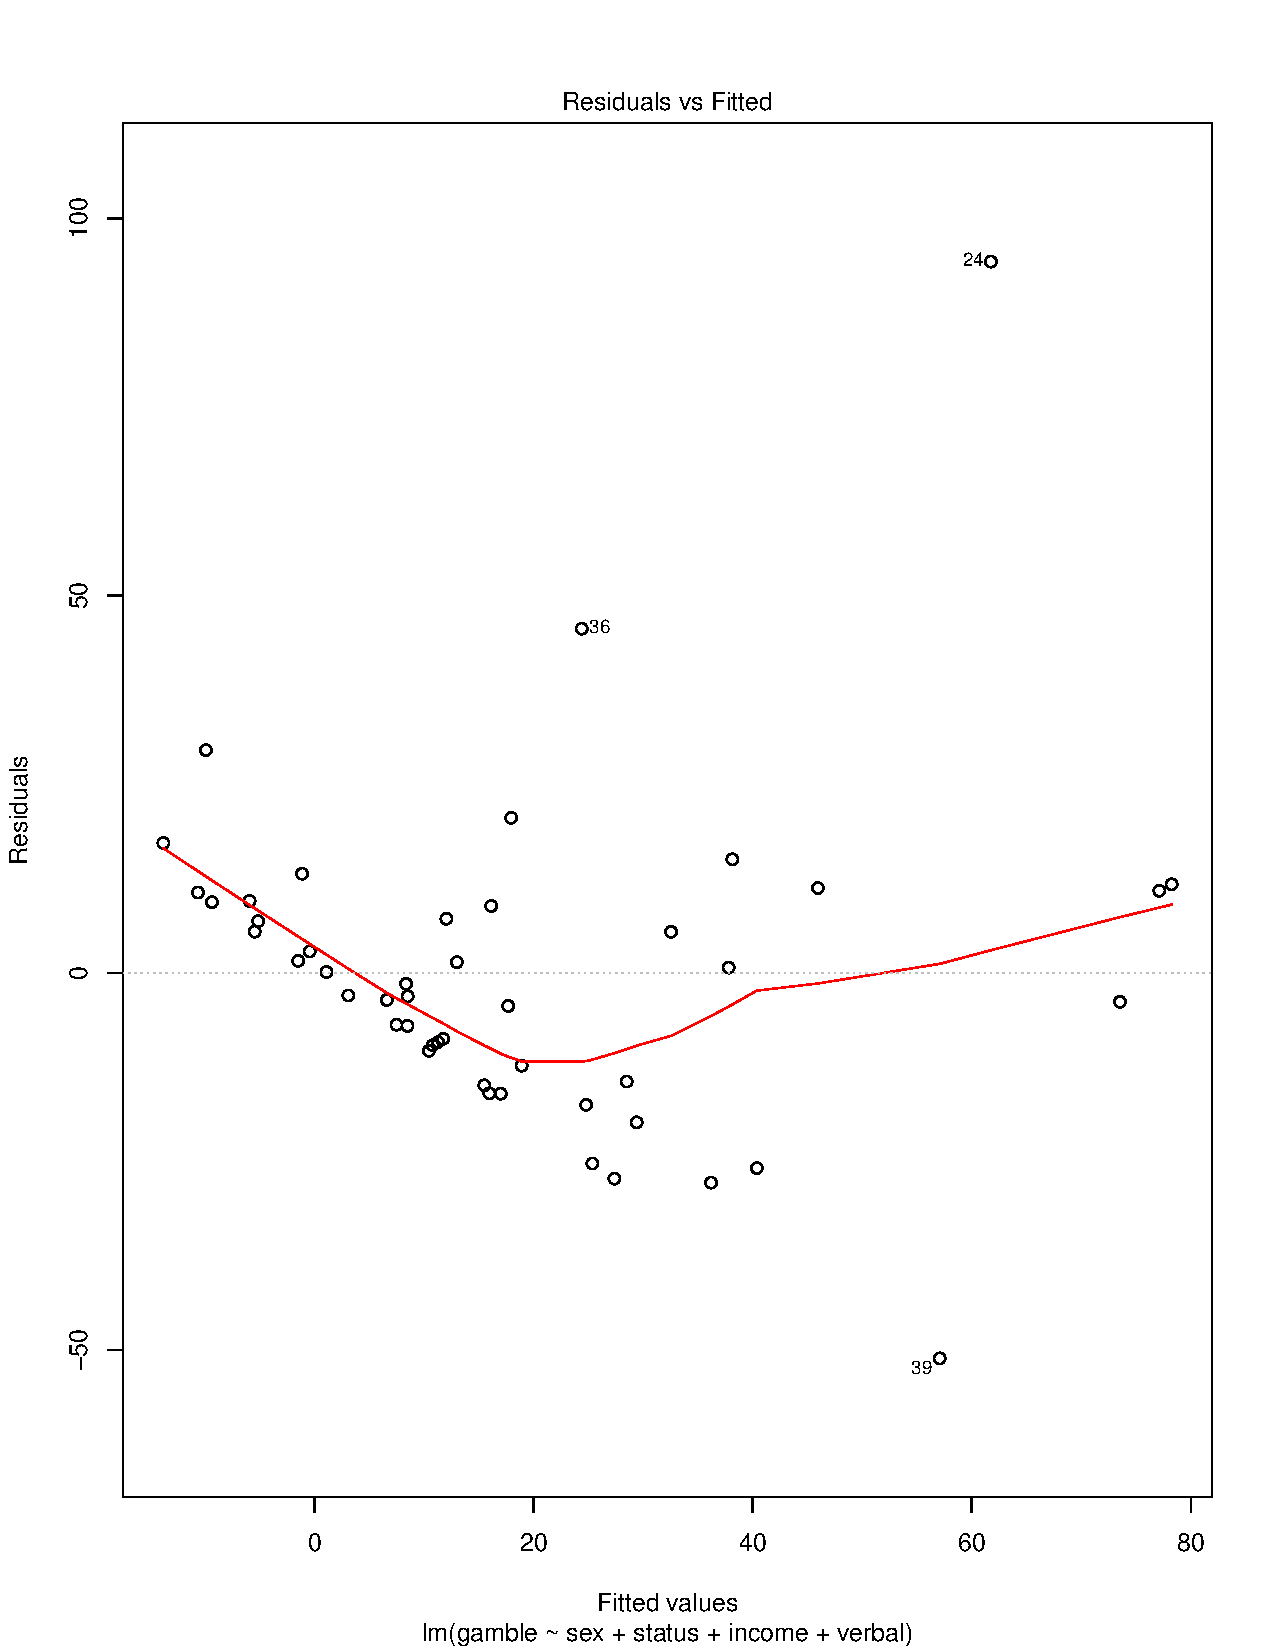
\includegraphics[width=.75\textwidth]{resid_fitted_pdf.pdf}\\
	 \end{figure}
	 
Constant variance illustrates the individual error against the predicted value, as the variance of the errors should be constant. Our plot isn't the cleanest, but overall would show a general trend of constant variance for most of the value points. There are some existing outlier values however, as indicated by the label above their data point, and distance from the residual axis of 0. 
	 
	 \newpage
	\item Check the normality assumption with a Q-Q plot of the studentized residuals. \vspace{6cm}

 \begin{figure}[h!]\centering
		\caption{\footnotesize QQ Plot.
		}\vspace{-1cm}
		\label{fig:plot1_b}
		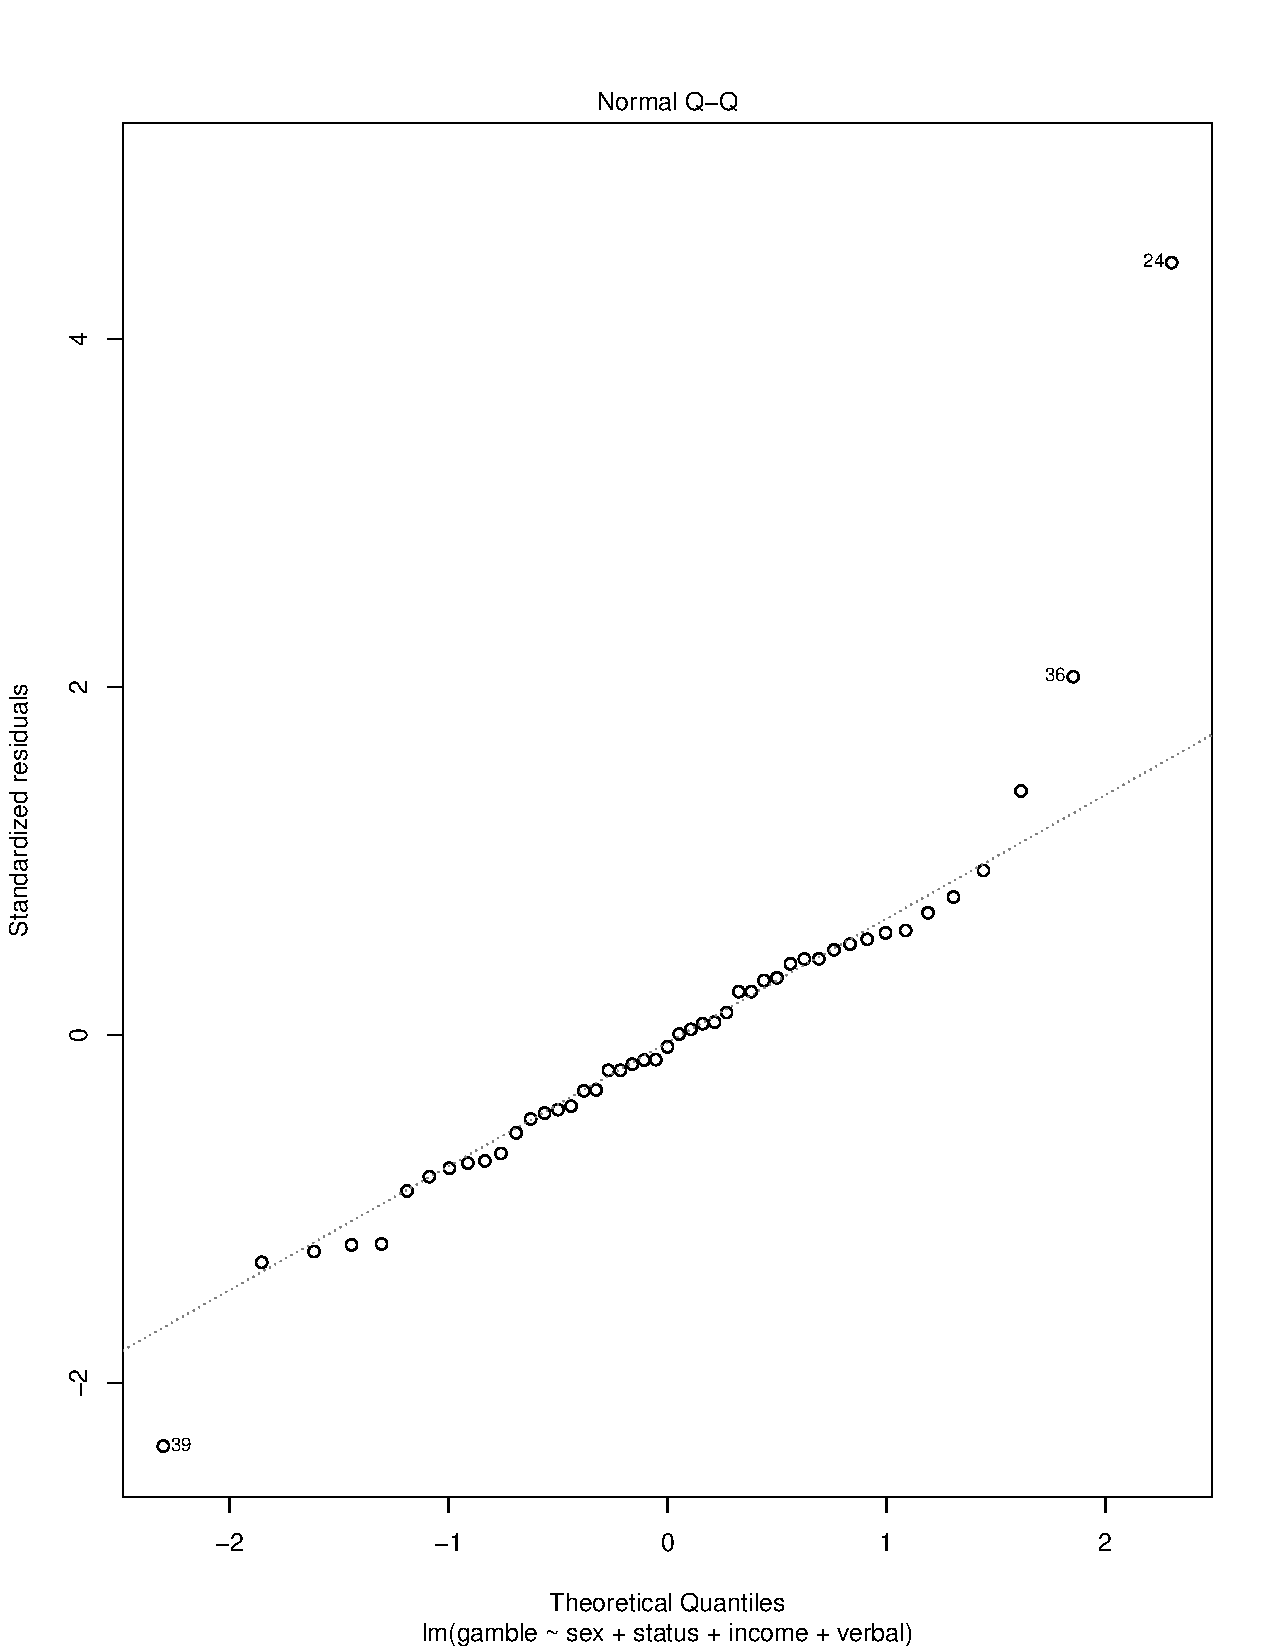
\includegraphics[width=.75\textwidth]{qq_plot_pdf.pdf}\\
	\end{figure}

A QQ-plot illustrates the distribution of the data against the expected normal distribution, and normally distributed data will exist on the straight line. On a general trend, we see that there is a relatively approximate straight line with the data points aside from about three data points. A curvature of these data points would indicate that the data is not normal, but at a holistic view, this data seems relatively normal. 


	\item Check for large leverage points by plotting the $h$ values. \vspace{6cm}
	
	 \begin{figure}[h!]\centering
		\caption{\footnotesize Residual vs Leverage Plot.
		}\vspace{-1cm}
		\label{fig:plot1_c1}
		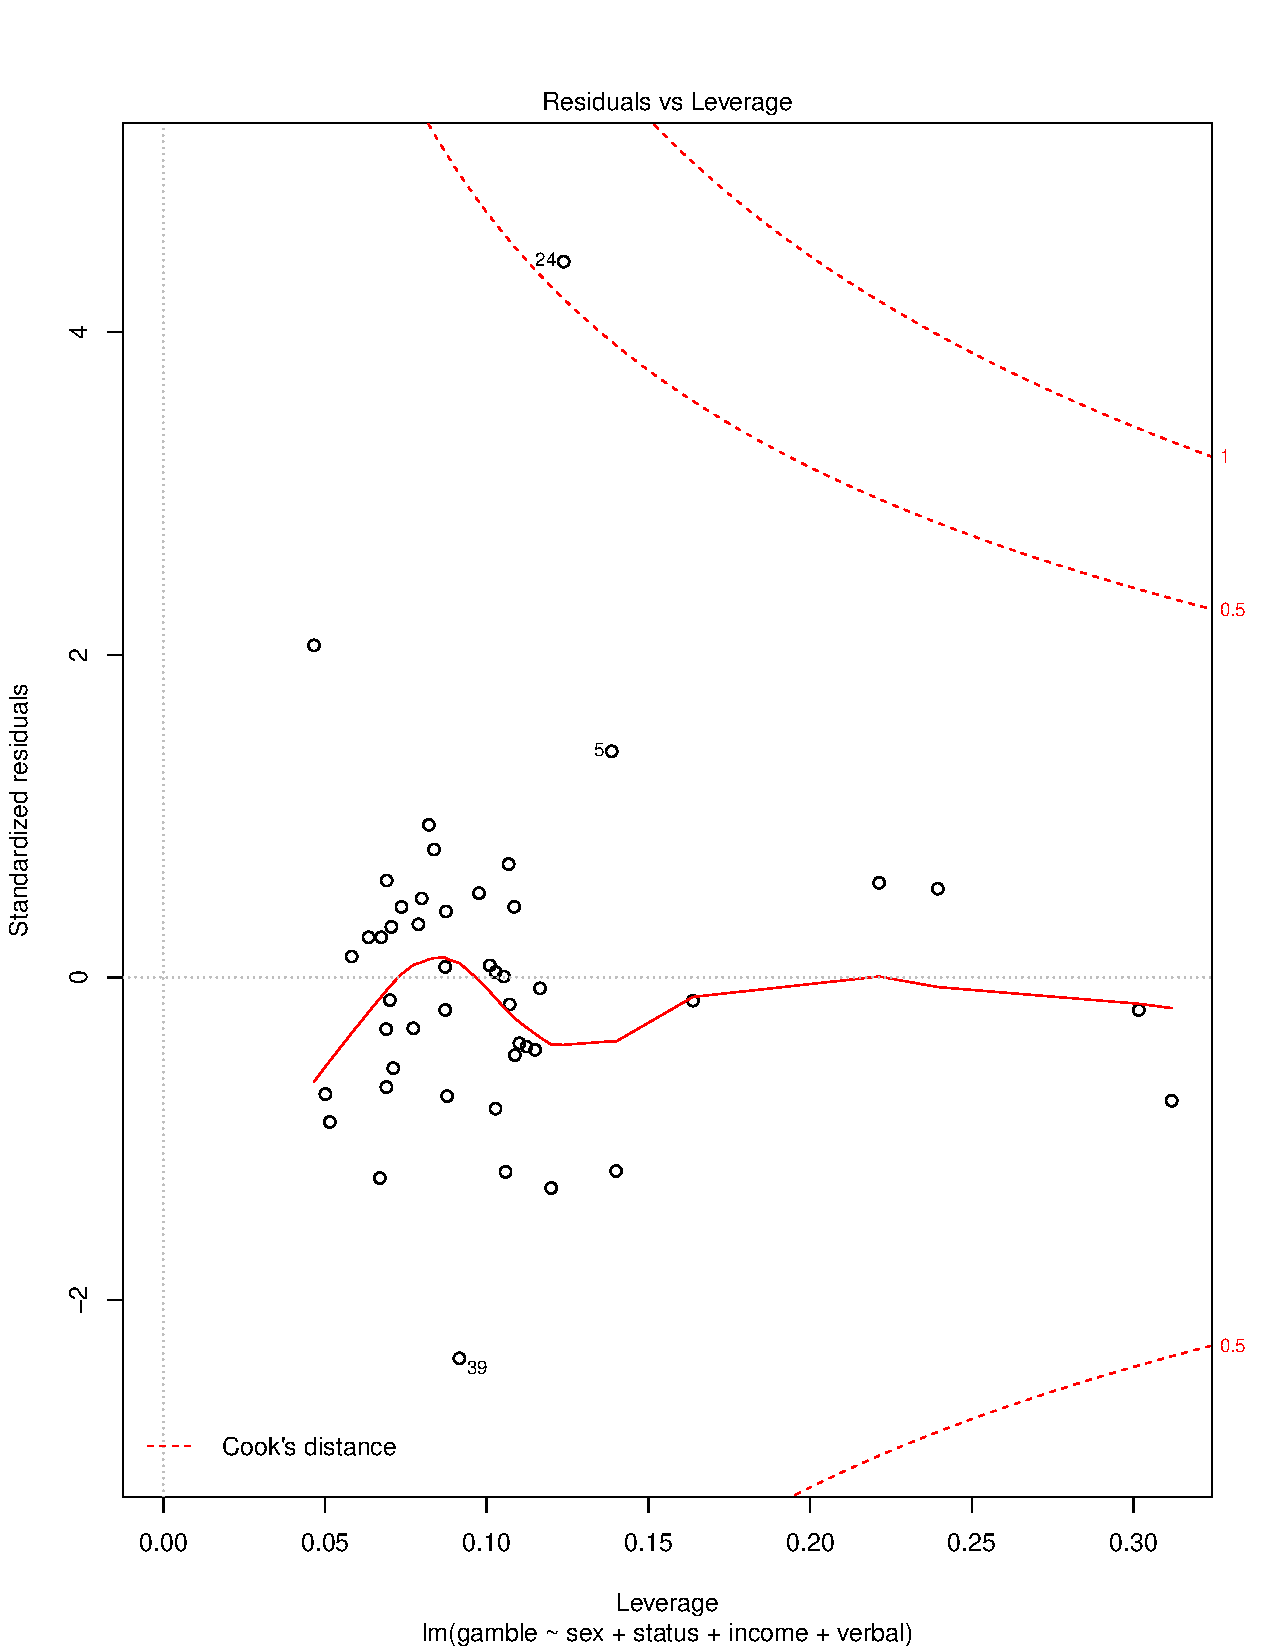
\includegraphics[width=.75\textwidth]{resid_leverage.pdf}\\
	\end{figure}

 \begin{figure}[h!]\centering
	\caption{\footnotesize Cook's Distance Plot.
	}\vspace{-1cm}
	\label{fig:plot1_c2}
	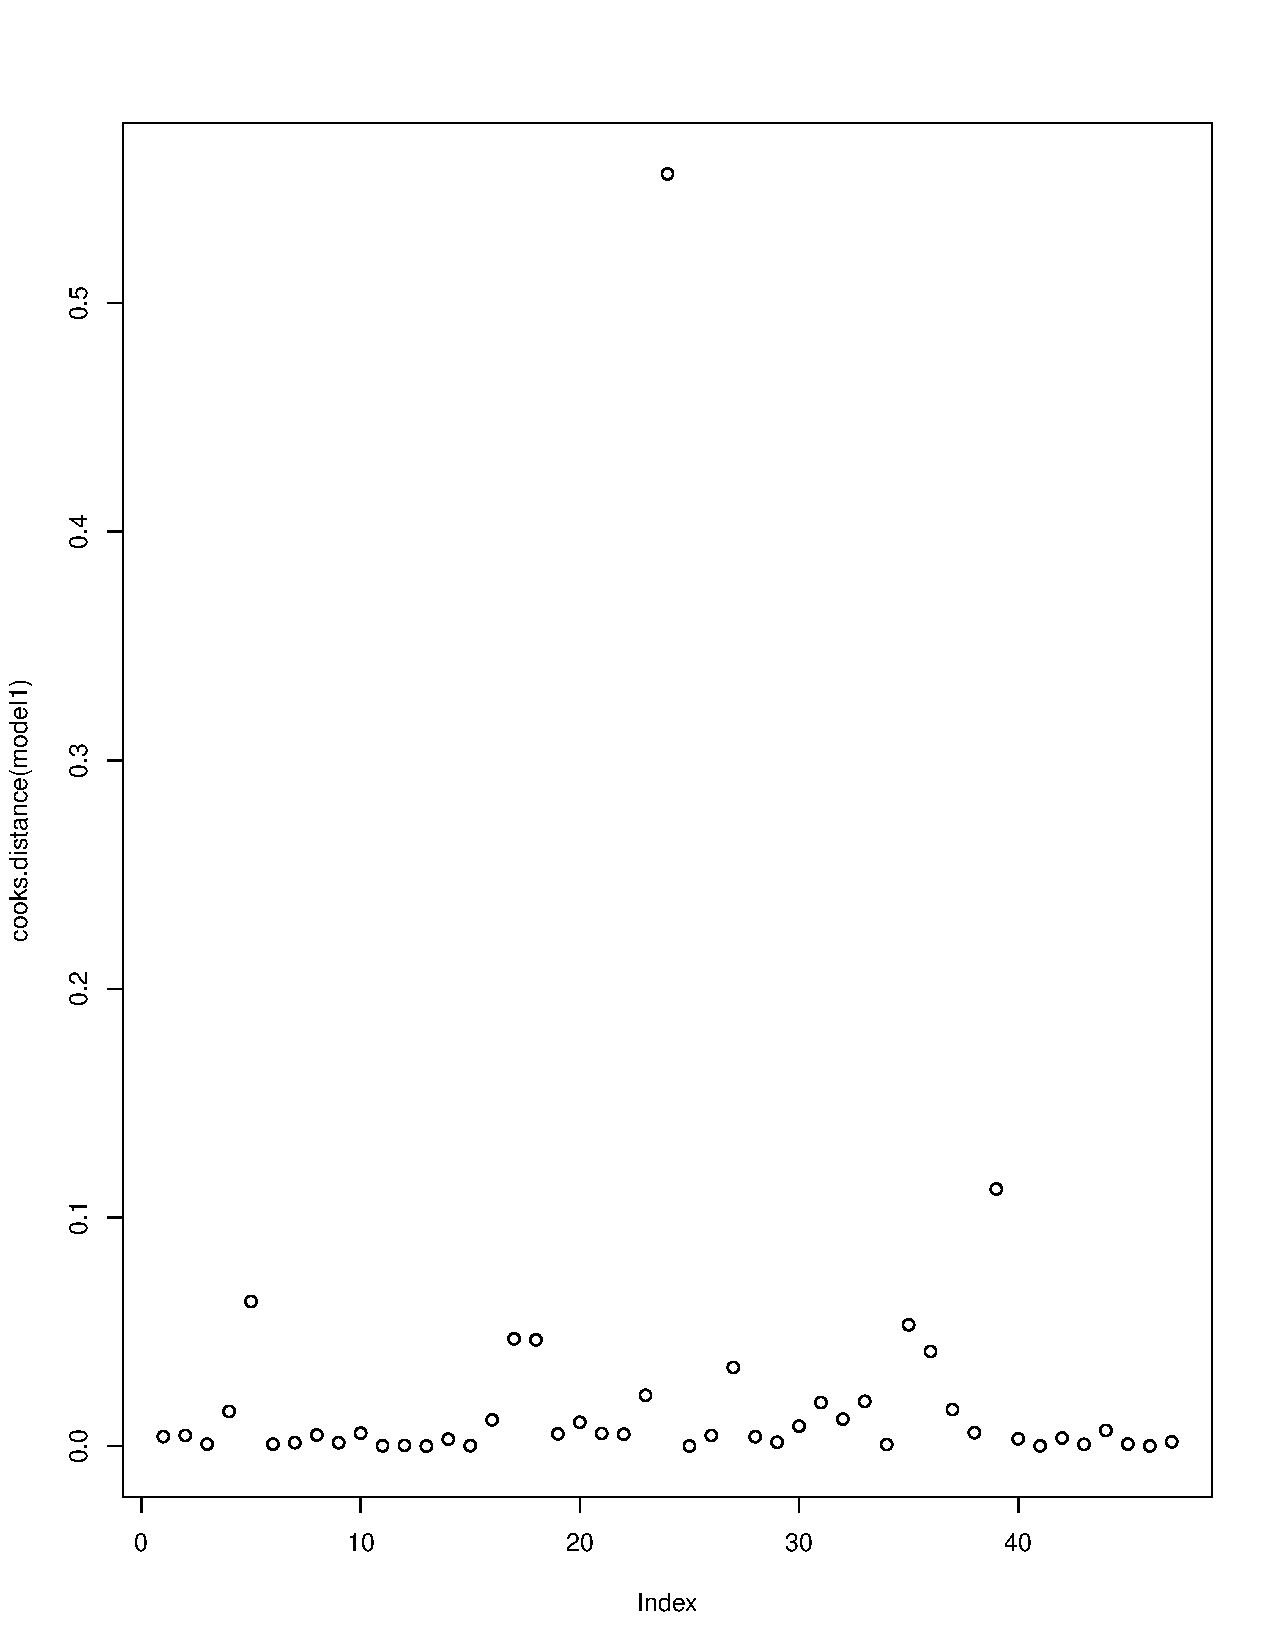
\includegraphics[width=.75\textwidth]{cooks_dis.pdf}\\
\end{figure}
\newpage
In these plots, we can see where the outliers exist, especially when observing Cook’s distance. Cook's distance shows the influence of each observation on the fitted response values, and can identify an outlier based on it's distance from the axis. There seems to be outlier values through these plots due to this great distance.

\newpage	
	\item Check for outliers by running an \texttt{outlierTest}. 
	
	\lstinputlisting[language=R, firstline=34, lastline=35]{PS5_Rcode.R} 
	
The value at 24, has a large studentized residual above 6, an unadjusted p-value is 4.1041e-07 while Bonferroni p-value is 1.9289e-05. Because it is smaller than a p-value of .05, we reject the null and conclude that in this model, the value 24 in the gamble dataset, is an extreme residual

\vspace{1cm}
	
	\item Check for influential points by creating a "Bubble plot" with the hat-values and studentized residuals.
	
	\lstinputlisting[language=R, firstline=38, lastline=44]{PS5_Rcode.R}  
	
	 \begin{figure}[h!]\centering
		\caption{\footnotesize Bubble Plot.
		}\vspace{-1cm}
		\label{fig:plot1_e}
		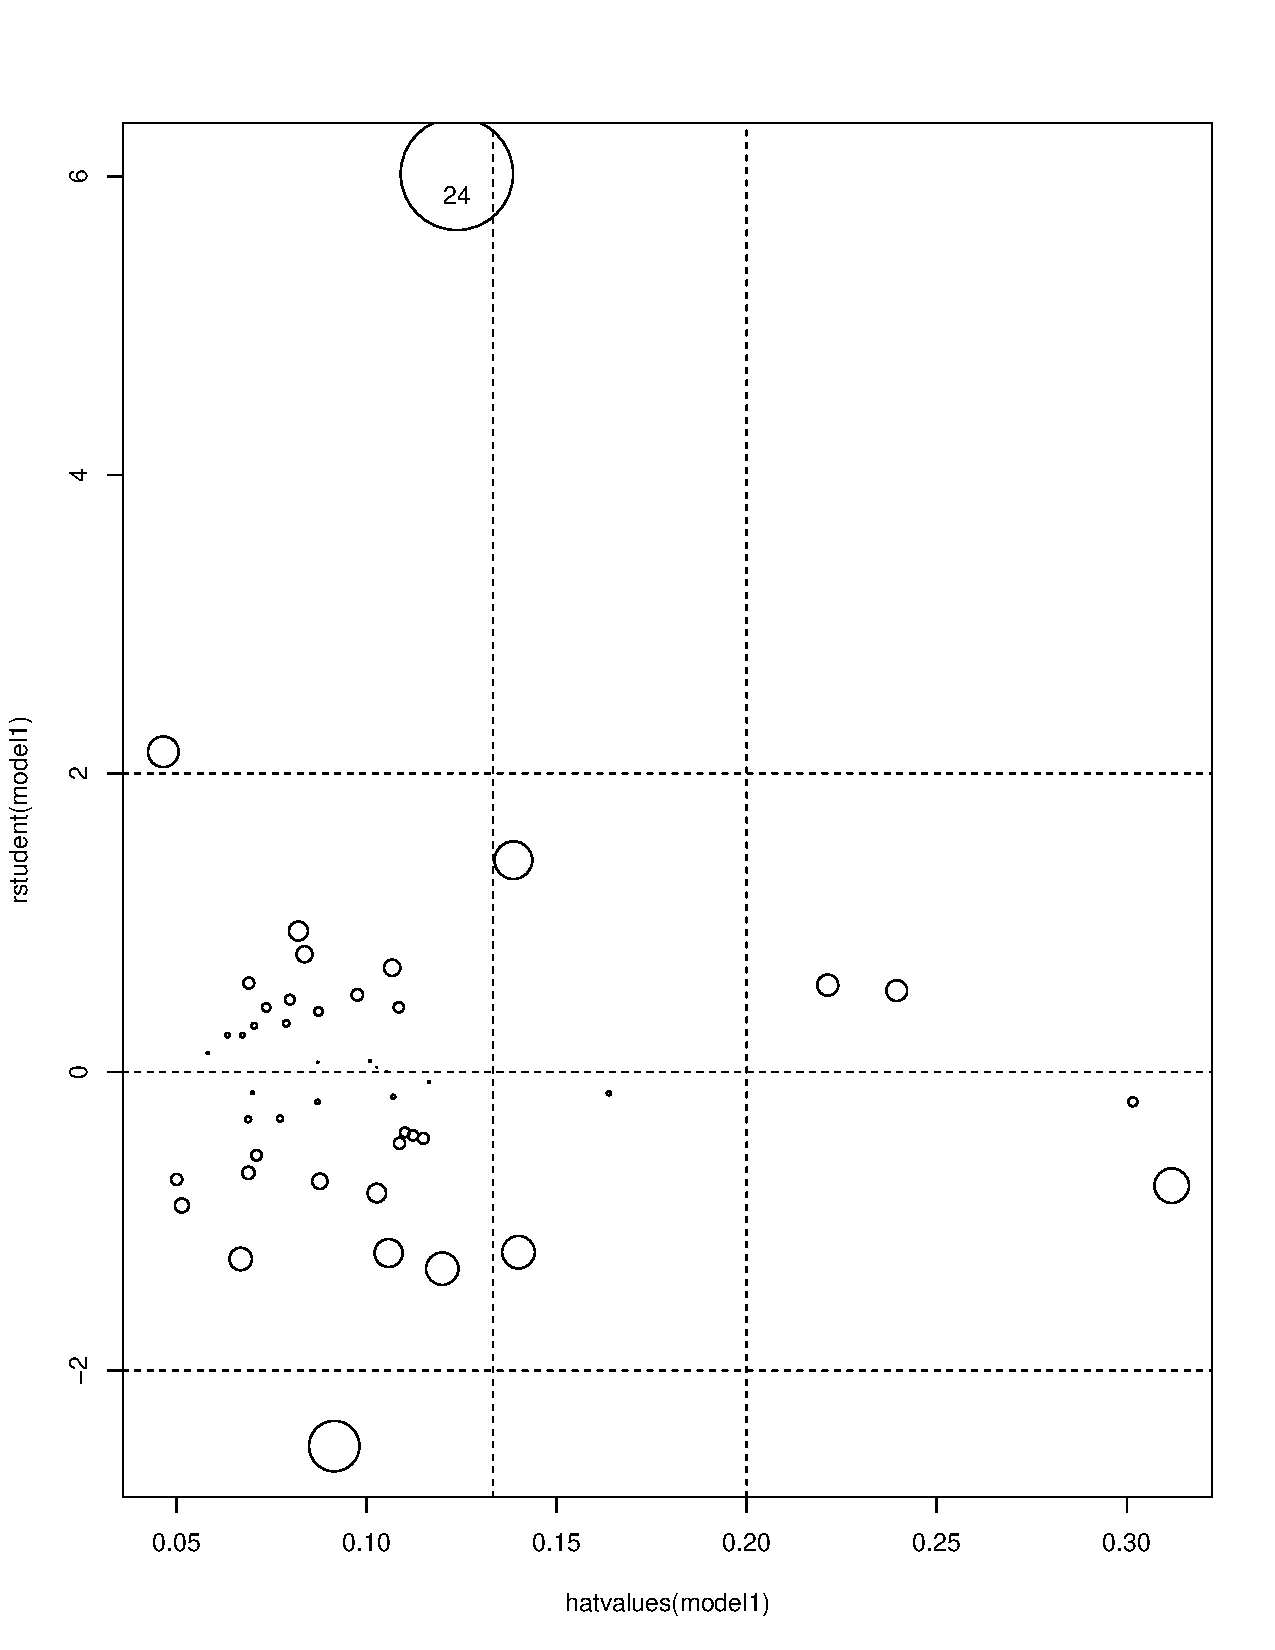
\includegraphics[width=.55\textwidth]{bubble_plot_labeled.pdf}\\
	\end{figure}
	% \item N/A.
\end{enumerate}

\end{document}
